\documentclass{article}
\usepackage{graphicx}
\topmargin=0.0in %length of margin at the top of the page (1 inch added by default)
\oddsidemargin=0.0in %length of margin on sides for odd pages
\evensidemargin=0in %length of margin on sides for even pages
\textwidth=6.5in %How wide you want your text to be
\marginparwidth=0.5in
\headheight=0pt %1in margins at top and bottom (1 inch is added to this value by default)
\headsep=0pt %Increase to increase white space in between headers and the top of the page
\textheight=9.0in %How tall the text body is allowed to be on each page
\newcommand\tab[1][3cm]{\hspace*{#1}}
\begin{document}
	
	\begin{center}
		{
			\Large\textbf{Akshit Gandhi}
		}
		
	\end{center}
	
	\begin{flushleft}
		1001,Radha Vishweshwar, 		\hspace{2.8in}    		    Contact: +91-9892558009            \\
		Narsing Lane, 		\hspace{2.85in}		    e-mail-id: akshitgandhi999@gmail.com \hspace{2.8in}
		Malad West, \\
		Mumbai-400064.     \\
		Maharashtra.\\
		
	\end{flushleft}
	\vspace{-0.3in}
	\begin{figure}[h]
		{%
		\hspace{4.4in}
\setlength{\fboxsep}{2.5pt}%
\setlength{\fboxrule}{1pt}%
\fbox{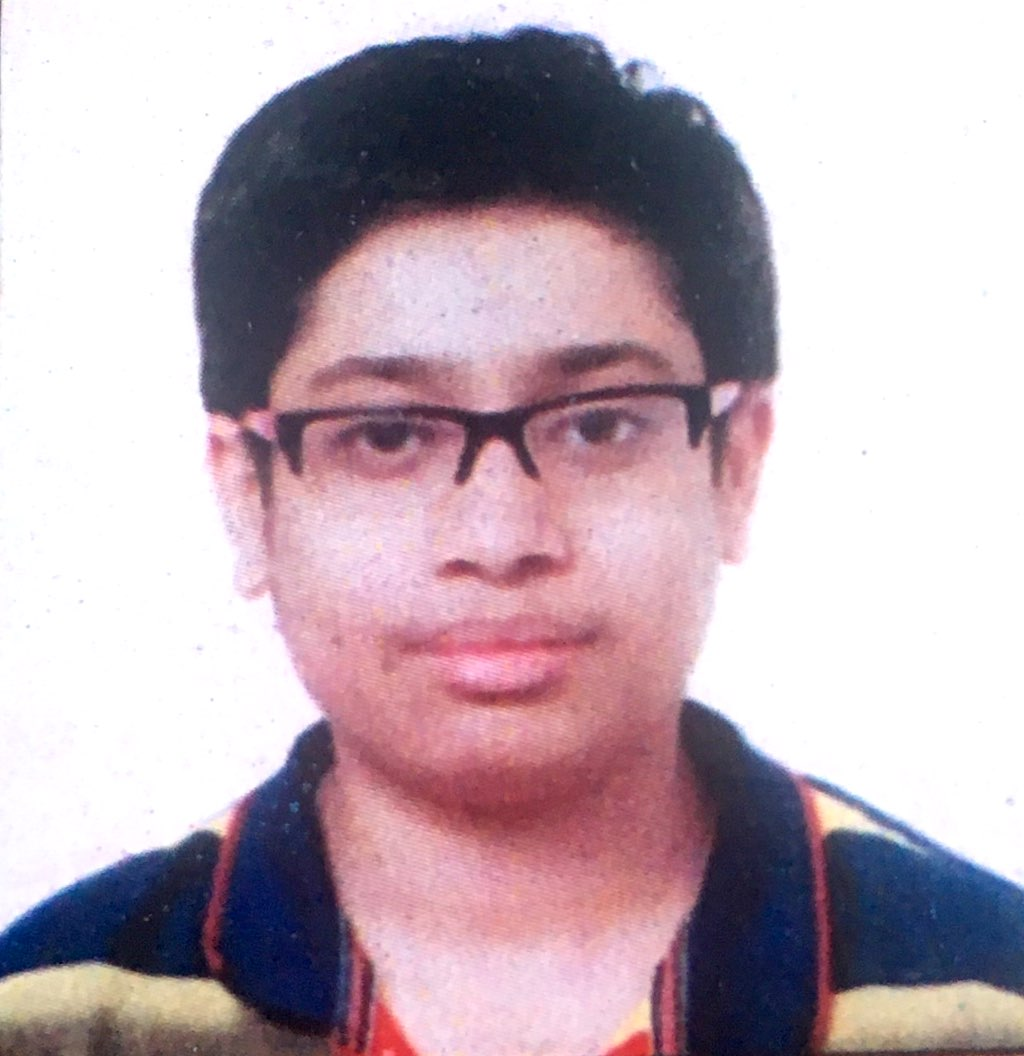
\includegraphics[width=3.5cm]{akshit}}%
}%
		\begin{flushleft}
\textrm{\textbf{Objective}}\\
\textrm{To learn more about embedded systems and use that knowledge to solve practical real-world problems. The main objective is to put whatever I learn, to practical use and solve problems faced in day to day life.}
\end{flushleft}
	\end{figure}
	
\begin{flushleft}
		
		\textbf{Education}
	\end{flushleft}
	
	\begin{tabular}{|c|c|c|c|c|}
		\hline
		\textbf{Degree} & \textbf{School/College} & \textbf{Board/University} &  \textbf{Year of passing} & \textbf{Pass}   \\
		&        &            &              & \textbf{Percentage}\\
		\hline
		
		S.S.C & Infant Jesus & Maharashtra Board & 2012 &90.55 \\
		Examination&School, Mumbai & & & \\
		\hline
		H.S.C& A.A.V.Patel& Maharashtra Board & 2014 &87.07 \\
		Examination&Jr. College, Mumbai& & & \\
		\hline
		B.Tech & V.J.T.I, & Mumbai University  & 2018 &8.97 CGPA\\
		(Computer Engineering)	&Mumbai &(Autonomous) & &(Till third \\
		(Pursuing)& && &Semester) \\
		\hline
	\end{tabular}
	\begin{flushleft} 
	 	\vspace{0.2in}
	 	\textbf{Projects}
	 	\begin{enumerate}
	 		\vspace{-0.29in}
	 		\addtolength{\itemindent}{1.359in}
	 		\item  Floor tiles that generate electricity using pressure.
	 		\item  Working on Quadcopter that can be interconvertible into a jet plane.
	 		\item  E-Yantra Robotics project on Hazardous Waste Disposal Theme\\ \hspace*{3.5cm}in eYRC-2015. 
	 	\end{enumerate}
	 \end{flushleft}
	\begin{flushleft}
	   	\vspace{1.15in}
	   	\textbf{Technical  \\ Skills}
	   	\begin{itemize}
	   		\vspace{-0.45in}
	   		\addtolength{\itemindent}{1.359in}
	   		\item  Familiar with the following Programming Languages .
	   		{\begin{itemize}
	   				\addtolength{\itemindent}{1.359in}
	   				\item C language
	   				\item C++ language
	   				\item Java 	
	   			\end{itemize}
	   		}  
	   		\item Knowledge of following micro controllers.
	   		{\begin{itemize}
	   				\addtolength{\itemindent}{1.359in}
	   				\item KK multicopter flight controller
	   				\item ATMEGA2560 Microcontroller	
	   			\end{itemize}
	   		}  
	   		
	   		\item Familiar with following Simulation Software
	   		{\begin{itemize}
	   				\addtolength{\itemindent}{1.359in}
	   				\item Atmel Studio 	
	   			\end{itemize}
	   		} 
	   	\end{itemize}
	   \end{flushleft}
	   
	   \begin{flushleft} 
	     	 		
	     	 		\vspace{0.4in}
	     	 		\textbf{Soft Skills}
	     	 		\begin{enumerate}
	     	 			\vspace{-0.30in}
	     	 			\addtolength{\itemindent}{1.359in}
						\item Teamwork 	     	 			
	     	 			\item Leadership
	     	 			\item Communication  
	     	 			\item Management
	     	 		\end{enumerate}
	     	 	\end{flushleft}
	     	 	
	\end{document}